\documentclass[11pt,a4paper]{article}
\usepackage[margin=25mm]{geometry}
\usepackage{fontspec}
\setmainfont{TeX Gyre Pagella}
\setsansfont{TeX Gyre Heros}
\setmonofont[Scale=0.86]{DejaVu Sans Mono}
\usepackage{amsmath,amssymb,booktabs,longtable,array,xcolor}
\usepackage{fvextra}
\usepackage{tikz}
\usetikzlibrary{arrows.meta,positioning}
\usepackage{xurl}
\usepackage[colorlinks=true,linkcolor=blue!45!black,urlcolor=blue!45!black]{hyperref}
\hypersetup{pdftitle={Chaining in CeTTa: Goals, patterns, proofs and evidence},
  pdfsubject={A runnable guide to HE and PeTTa chaining and directional matching}}
\usepackage{microtype}
\definecolor{codebg}{RGB}{246,247,249}
\DefineVerbatimEnvironment{code}{Verbatim}{fontsize=\small,breaklines=true,
  breakanywhere=true,frame=single,rulecolor=\color{black!20},framesep=3mm}
\newcommand{\src}[1]{\VerbatimInput[fontsize=\small,breaklines=true,
  breakanywhere=true,frame=single,rulecolor=\color{black!20},framesep=3mm]{#1}}
\NewDocumentCommand{\name}{v}{\texttt{#1}}
\newcommand{\file}[1]{\par\smallskip\noindent\textsf{\small\detokenize{#1}}\par\smallskip}
\setlength{\parindent}{0pt}
\setlength{\parskip}{6pt}
\setcounter{tocdepth}{2}
\title{Chaining in CeTTa\\\large Goals, patterns, proofs and evidence}
\author{A runnable guide for HE and PeTTa programs}
\date{7 October 2026}
\begin{document}
\maketitle

A chainer connects facts to questions. A useful chainer also tells us which
facts supported its answer, how much search it was allowed to perform, and
whether an unanswered question was disproved or merely not reached.

This guide builds a small proof-producing backward chainer, a forward closure,
and programmable search gates. It then adds directional matching, joint
constraints, loop tests and occurrence-sensitive evidence. The final chapters
connect these pieces to Nil Geisweiller's proof-size search and
backward-via-forward experiments, and to the existing PLN examples.

The examples use CeTTa's HE and PeTTa dialects. Their common notation is useful,
but the dialects are not interchangeable. Differences that affect a program
are marked explicitly. The \name{pat} operations are CeTTa extensions; importing
this module into another implementation does not install a native matcher there.

\begin{center}
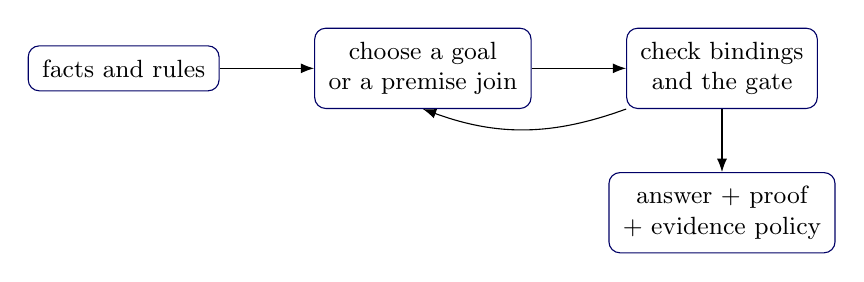
\begin{tikzpicture}[node distance=8mm and 12mm,>=Latex,
 box/.style={draw=blue!40!black,rounded corners,align=center,inner sep=5pt,font=\small}]
\node[box] (facts) {facts and rules};
\node[box,right=of facts] (choice) {choose a goal\\or a premise join};
\node[box,right=of choice] (match) {check bindings\\and the gate};
\node[box,below=of match] (proof) {answer + proof\\+ evidence policy};
\draw[->] (facts)--(choice); \draw[->] (choice)--(match);
\draw[->] (match)--(proof); \draw[->] (match.south west) to[bend left=20] (choice.south);
\end{tikzpicture}
\end{center}

\newpage
\tableofcontents
\newpage
\section{Quick start}

\paragraph{Build.} CeTTa is a C program. On Debian or Ubuntu, install the
build dependencies and build the default binary from the repository root:
\begin{code}
sudo apt install build-essential pkg-config python3-dev libgmp-dev
make
\end{code}
This produces \name{./cetta}. GMP provides exact big integers; build with
\name{make ENABLE_GMP=0} to do without it. SWI-Prolog is detected
automatically when present and is optional. The repository's README lists the
other build modes.

\paragraph{Run.} All commands below run from the repository root. Every
example names its dialect and profile:
\begin{code}
./cetta --lang he --profile extended examples/chaining/tutorial/01-backward.metta
./cetta --lang petta --profile extended examples/chaining/tutorial/01-backward.metta
\end{code}
The \name{pat} operations and \name{=%} rules belong to the \name{extended}
profiles. Their names stay ordinary data in other profiles.
This backward-chaining example also runs in plain PeTTa.

\paragraph{Check.} One command runs the tutorial and its companion SKI,
clause and PLN clients, and compares their answers, negative cases, variable
aliasing and evidence occurrences with the expected results:
\begin{code}
make BUILD=python test-chaining-tutorial
\end{code}

\paragraph{Read the output.} HE prints the answers of each \name{!}
expression as one bracketed list; PeTTa prints each answer on its own line.
\name{collapse} gathers all alternatives into one expression. HE's \name{[()]}
after a collapsed failed search is therefore one empty collection, not an
absence of answers. Import and include forms also print their dialect's setup
result; the discussion below concerns the queries that follow them.

Appendix~\ref{app:card} is a one-page reference card for the matching
operations.

\section{Start with a question and a proof}

Our first knowledge base is deliberately small:
\file{examples/chaining/tutorial/graph-facts.metta}
\src{examples/chaining/tutorial/graph-facts.metta}

\name{fact}, \name{rule} and \name{proof} are ordinary data constructors
chosen by this program. They are not new language primitives. Each fact has
a label; each rule has a list of premises and a conclusion.

The question \name{(reachable alice dana)} needs three edges. An answer such
as \name{True} would hide that reasoning. Instead, a leaf proof records its
fact label, while a rule proof records its rule name and child proofs.
For instance:
\begin{code}
(proof (direct ((proof ab (edge alice bob))))
       (reachable alice bob))
\end{code}
A consumer can walk this tree and check each rule against the same knowledge
base. Merely printing a value called \name{proof} is not independent proof
checking: the producer and any checker still need a stated rule semantics.

\section{Backward chaining with an explicit gate}

Backward search starts with a desired conclusion. It tries a matching fact,
then rules whose conclusions can unify with that goal. For a rule, it solves
all premises in one shared environment. This is why the middle vertex of a
path is the same in both premises.

\file{examples/chaining/tutorial/backward-core.metta}
\src{examples/chaining/tutorial/backward-core.metta}

Read \name{bc} as follows. First ask the gate whether this search is allowed.
Then choose a fact or a rule. A fact returns a leaf proof. A rule recursively
proves its premises and returns a node whose children are those proofs.
\name{bc-all} threads the ordinary bindings through the premise list using
\name{let*}. A failed premise produces no proof for that rule application.

The gate is checked again after a fact is selected or the premises are solved.
This matters: a goal such as \name{(edge bob $to)} is less informative than
the resulting \name{(edge bob carol)}. A policy that rejects the latter cannot
rely solely on the earlier open goal.

Ordinary \name{match} is intentional here. A query with an unknown destination
should discover it; a stored rule's variables should become related to the
caller's variables. Replacing every \name{match} by directional matching
would change this relational algorithm.

\file{examples/chaining/tutorial/01-backward.metta}
\src{examples/chaining/tutorial/01-backward.metta}

The four observations are:
\begin{enumerate}
\item With depth four, Alice reaches Dana with a nested \name{step},
\name{step}, \name{direct} proof.
\item Depth three is insufficient, so the collapsed answer is empty.
\item With depth two and an open destination, the answer is Bob with its
direct proof.
\item Dana has no outgoing edge, so the last search returns no proof.
\end{enumerate}

The depth counts the longest nested proof path in this implementation,
including a fact leaf. It does not count all nodes in a branching proof.
Each sibling receives the same remaining depth. Section~\ref{sec:nil} shows
Nil's different, proof-size accounting.

On a finite knowledge base with finite premise lists and a fixed finite depth,
this client has a finite search tree. Increasing the bound can expose new
proofs. An empty result at one bound establishes only failure within that
bound, not logical falsity.

\section{Binding direction is independent of search direction}

``Forward'' and ``backward'' search concern where reasoning starts.
Directional matching concerns which variables a single comparison may bind.
A forward chainer and a backward chainer can each use either binding policy
where appropriate.

For a pattern $p$ and a subject $s$, a directional match seeks a substitution
$\sigma$ such that
\[
  \sigma(p)=s,\qquad \sigma(x)=x\quad\text{for every variable of }s.
\]
The subject may contain variables. Protecting them is precisely what makes
this different from matching only ground data. Ordinary unification instead
seeks $\sigma(p)=\sigma(s)$ and can instantiate variables on both sides.

\begin{center}
\begin{tabular}{lll}
\toprule
Pattern & Subject & Directional result\\\midrule
\name{(pair $x $x)} & \name{(pair a a)} & $x\mapsto a$\\
\name{(pair $x $x)} & \name{(pair a b)} & failure\\
\name{(pair $x $x)} & \name{(pair $u $u)} & $x\mapsto u$, $u$ unchanged\\
\name{(pair $x $x)} & \name{(pair $u $v)} & failure for distinct $u,v$\\
\bottomrule
\end{tabular}
\end{center}

The percent sign marks the \emph{protected} side. In \name{pat:match%} the
stored subject is protected and the query pattern binds; in \name{pat:%match}
the query is protected and the stored patterns bind; in a \name{=%} rule the
caller is protected and the rule head binds.

Readers who know Prolog will recognise the relations: \name{pat:is-instance t p}
corresponds to ISO \name{subsumes_term(p, t)}, which likewise leaves the
specific term's variables unchanged even when the two terms share variables, and
\name{pat:is-variant} corresponds to SWI-Prolog's \name{=@=}.

Import one module:
\begin{code}
!(import! &self pat)
\end{code}
The everyday calls keep their \name{pat:} prefix and return templates directly.

\file{examples/chaining/tutorial/02-direction.metta}
\src{examples/chaining/tutorial/02-direction.metta}

The three stored edges include an open row and two equal ground rows.
Ordinary \name{match} produces three destinations: it may instantiate the
open stored variable. \name{pat:match%} produces two: only its query pattern
may bind, so that open row cannot be changed into \name{(edge a b)}.
Both copies of the ground row remain separate answers.

\name{pat:%match} asks the converse retrieval question: which stored patterns
cover this fixed term? Its extra binder names the original stored row, so the
template can report it. In this example it returns all three rows. It does
not mean executing a rule backwards. The binding permission has changed;
the rule's conclusion and premises have not exchanged roles.

\begingroup\small
\begin{longtable}{p{.51\linewidth}p{.43\linewidth}}
\toprule Form & Contract\\\midrule
\name{pat:match% space pattern template} & Retrieve with stored subjects
protected; instantiate and evaluate the template for each hit.\\
\name{pat:%match space term output template} & Retrieve covering stored
patterns; protect the query term and bind \name{output} to the original row
(or tuple of rows for a conjunction).\\
\name{pat:let% pattern producer body} & Evaluate the producer, match each
result directionally, then evaluate the body with those bindings.\\
\name{pat:case% producer branches} & Evaluate the producer and use
directional branch matching under the dialect's case control contract.\\
\name{pat:unify% pattern subject yes no} & Match raw syntax, then choose the
success or failure continuation.\\
\name{pat:is-instance term pattern} & Test whether the pattern can become
the fixed term. Return a dialect Boolean, without exporting a substitution.\\
\name{pat:is-variant a b} & Test whether one consistent bijection of logic
variable identities turns one term into the other.\\
\bottomrule
\end{longtable}
\endgroup

The raw tests do not evaluate a call expression merely because it occurs in
an operand. To compare a computed value, bind that value first with ordinary
\name{let}. For example, the loop test in Section~\ref{sec:loops} computes
\name{car-atom} before calling \name{pat:is-variant}.

Protection belongs to the matching attempt. It is not a lasting prohibition
on future ordinary unification in the body. A successful match can return an
open term whose variable is later bound by an explicit ordinary operation.

\section{Forward chaining as controlled closure}

Forward search starts from known facts and joins premises to derive more
facts. Here \name{reach(x,y)} and \name{edge(y,z)} imply \name{reach(x,z)}.
The shared variable $y$ makes this a join, rather than an arbitrary pair of
facts.

\file{examples/chaining/tutorial/03-forward.metta}
\src{examples/chaining/tutorial/03-forward.metta}

This client chooses \emph{set-valued reachability}. Before insertion it checks
whether the ground fact is already present. The matching API itself still
preserves duplicates. A proof-enumerating chainer might instead keep several
derivations of the same conclusion; that is a different evidence policy.

Each round first collects its candidates and then inserts them. Consequently,
a new fact cannot unexpectedly become an input midway through that round.
One round reaches Bob and Carol from Alice; the next also reaches Dana.
A third round changes nothing. The negative query from Dana to Alice remains
empty. This is a bounded, explicit closure client, not a transactional worker
system or an implicit fixed-point primitive.

For a larger application, replace the repeated full scan with a delta agenda:
enqueue newly admitted facts, join them with the existing index, and enqueue
only new consequences. Keep the choice of duplicate policy explicit. The
incremental matcher described later reuses a \emph{query's prefix}; it is not
by itself such a whole-program agenda.

\section{Programmable gates without accidental guessing}

A gate is an ordinary program supplied to the chainer. It can inspect a goal,
the remaining budget, or a context value threaded by a richer chainer.
Directional tests are useful because inspecting a goal need not refine it.

\file{examples/chaining/tutorial/04-gates.metta}
\src{examples/chaining/tutorial/04-gates.metta}

The first query allows the Alice--Dana proof. The second excludes the
Bob--Carol premise and therefore returns no proof. The third still permits
Alice--Bob. This policy intentionally sacrifices completeness relative to the
unrestricted knowledge base.

The gate's raw \name{pat:unify%} test does not fill an open endpoint just to
make it match the forbidden edge. The post-match gate check in \name{bc}
then rejects the forbidden edge when it has actually been selected.

Nil's inference-control clients go further: context updates and the pruning
predicate are arguments, and another chainer can prove a termination condition.
The standing benchmark includes such a nested controller. The architecture
does not require a new delayed-goal language to make a useful gate today.
An undecided, suspended logical guard would require an additional resumption
contract; this tutorial does not silently substitute a Boolean gate for it.

\section{Joint constraints and the scope of protection}

Some questions require several comparisons to agree on one substitution.
The number of comparisons is unrestricted by the notation; ``joint'' does
not introduce a different kind of variable for each arity.

\file{examples/chaining/tutorial/05-joint.metta}
\src{examples/chaining/tutorial/05-joint.metta}

The conjunction finds exactly \name{(grandparent alice carol)}. The three-pair
solver returns a witness that can instantiate \name{(proof $x $y)} to
\name{(proof a b)}.

The next pair family is the important negative example. Its first comparison
captures a subject variable; its second would have to change that protected
variable into \name{a}. The \emph{whole family} therefore fails.
Nested \name{pat:let%} forms are separate attempts. The inner attempt may
have a different protected set, so the following nested example returns
\name{(separate a)}. Use a conjunction or \name{pat:solve} when all comparisons must agree under
one protected set.

The advanced basis has four operations:
\begin{description}
\item[\texttt{pat:solve}] Solve a list of term pairs under \name{match%},
\name{%match}, \name{unify} or \name{variant}, and return a reusable witness.
\item[\texttt{pat:apply}] Apply that witness to syntax. This lets a client build
several outputs from one solved constraint family.
\item[\texttt{pat:view}] Inspect the complete variable map. An interactive
constraint tool receiving arbitrary input pairs does not know their variable
domain in advance; a fixed application template cannot list that domain.
\item[\texttt{pat:query}] Retrieve rows together with their occurrence identities
and a witness. Use it when an answer's supporting rows are part of the result.
\end{description}
Normal template retrieval needs none of these records. A \name{Bindings}
value is an existing grounded substitution value, not a rule to interpret a
user-created expression with that printed name. Treat the witness as an
opaque value and use its operations.

For the solved pair family above, \name{pat:view} returns:
\begin{code}
(Bindings (($x a) ($y b)) ())
\end{code}
The first field lists assignments; the second retains residual equality
constraints. The final \name{()} means that none remain. Dropping that field
would hide obligations in a result that has residual constraints. This is
the existing bindings representation; ordinary template queries still return
their templates directly.

For a joint directional solve, subject variables from the entire family are
protected. Incremental execution must also notice a variable that becomes a
protected subject only in a later pair. The native prefix state checks that
case and refuses to revise an earlier image to force success.

\section{Loop tests, memoization and tabling}\label{sec:loops}

Two goals are variants when they have the same shape and the same variable
sharing, up to a one-to-one renaming. \name{(f $x $x)} and
\name{(f $u $u)} are variants; \name{(f $x $x)} and \name{(f $u $v)} are not.
This concerns free logic variables. It is distinct from alpha-equivalence
of bound variables in a higher-order language.

\file{examples/chaining/tutorial/07-loop-tests.metta}
\src{examples/chaining/tutorial/07-loop-tests.metta}

The answers are true, false, false, true. A ground destination is an instance
of an open destination, but they are not variants. Computing the ancestor
first is essential because the relation test inspects raw syntax.

For terms that share variable identities, protection also matters. The terms
\name{(f $x $y)} and \name{(f $y $x)} are variants. Neither can be turned into
the other by a substitution that fixes all variables of the specific operand.
Thus do not implement this protected instance predicate by assuming that
two independently tested directions always reproduce the variant predicate.

An ancestor check can prevent repeating a goal along one branch. It does not
show that all answers to that goal have been found. In particular, treating
an unfinished recursive call as a completed empty table can lose proofs.
Tabling manages dependencies and answer completion; memoization reuses
completed calls according to its cache contract.

\file{examples/chaining/tutorial/08-tables.petta.metta}
\src{examples/chaining/tutorial/08-tables.petta.metta}

This chapter uses the existing PeTTa libraries and works in plain PeTTa as
well as extended. \name{fib 20} returns 6765. The tabled duplicate proof has
one answer, while the ordinary duplicate equations have two. The missing
goal has no answer. Both memoized square calls return 81.

Coalescing table answers may be right for reachability and wrong for an
evidence bag. If different derivations must remain distinguishable, include
their proof or evidence identity in the tabled answer and choose the intended
semantics deliberately. Cache reuse for effectful or changing computations
also requires the library's invalidation and effect contract; the square
example is intentionally pure.

\section{Evidence you can inspect}

\file{examples/chaining/tutorial/06-evidence.metta}
\src{examples/chaining/tutorial/06-evidence.metta}

The first query returns two derivations of \name{(reachable alice carol)}.
Their first supporting rows have different occurrence identities, although
their labels and values are equal. Their second supporting row has the same
identity. The last query returns no certificate.

The record vocabulary is small:
\begin{code}
(pat:hit rows witness)
(pat:row occurrence original instantiated)
(pat:occurrence space-id revision row-id)
\end{code}
Rows appear in premise order. The identity refers to a row in a particular
space read, not a universal persistent evidence name. A program that needs
durable source identity should also store its own source labels and metadata.
The \name{original} row retains its pattern; the \name{instantiated} view
shows the selected match. Equal values can have different occurrences.

These identities make dependence visible. They do \emph{not} establish that
two observations are statistically independent, and they do not automatically
prevent double counting. In this example, both derivations share the second
observation. Any probabilistic revision must account for that overlap using
its own evidence model.

\subsection{Forward and backward clause subsumption}
For finite first-order clauses, $C$ subsumes $D$ when one substitution on
$C$ makes every literal of $C$ occur in $D$, preserving polarity. The choice
of literal correspondences is part of the search. It is more than testing
each literal independently.

\file{examples/pattern/clause_retrieval.metta}
\src{examples/pattern/clause_retrieval.metta}

Forward subsumption asks which old clauses cover the new one. Backward
subsumption asks which old clauses the new one covers. The optional
\name{pat:clause} module performs the clause search; it is not a module of
short aliases. The example retains two equal stored clauses as two evidence
occurrences even when both prove the same logical redundancy.

Set and multiset clauses have different contracts. Set coverage may reuse a
literal of the specific clause. Multiset coverage requires separate
occurrences. The positive set example and negative multiset example in this
file make that difference observable. A theorem about redundancy does not
itself authorize deleting evidence or changing a proof bag.

\subsection{PLN: choose premises before combining truth values}
Directional retrieval can select the premise topology of induction or
abduction while leaving evidence untouched. Induction often compares two
links with a common source; abduction compares links with a common target.
Those topologies do not turn matching itself into probabilistic inference.

The maintained client \name{examples/pattern/pln_selection.metta} selects
evidence and priors and builds a value named \name{selected}. Its dialect
wrappers import their existing PLN truth functions:
\begin{code}
./cetta --lang he --profile extended examples/pattern/pln_selection.he.metta
./cetta --lang petta --profile extended examples/pattern/pln_selection.petta.metta
\end{code}
The example includes an open fact that must not be instantiated to manufacture
a missing premise, and duplicate observations that remain duplicate selections.
It reports the truth-function inputs alongside the conclusion. The current
HE and PeTTa libraries use different confidence formulas; the client preserves
each library's result rather than claiming cross-dialect formula identity.

Use \name{pat:query} instead of value-only retrieval when a revision policy
needs occurrence identities. Keep separate the questions ``does this tuple
fit the inference schema?'' and ``what evidence model justifies combining
its truth values?''

\section{Nil's proof-size search and backward-via-forward search}\label{sec:nil}

Nil's optimized propositional chainer carries \name{(MkSized size proof)}.
An axiom costs one node. A modus-ponens proof combines an implication proof
of size $f$, an antecedent proof of size $x$, and one application node:
\[
  \operatorname{size}(\operatorname{mp}(F,X))=f+x+1.
\]
For a total allowance $s$, the implementation first reserves room for the
application and the second proof, then passes the actual remainder
$s-1-f$ to the second recursive call. This is not the depth bound from our
first chainer.

\file{examples/chaining/tutorial/09-nil-size.petta.metta}
\src{examples/chaining/tutorial/09-nil-size.petta.metta}

The included engine is the pinned source already used by the chainer ladder.
Zero budget rejects an axiom; one admits it. Four nodes cannot prove the
identity formula in this search; five produce
\begin{code}
(MkSized 5 (: (mp (mp ax₂ ax₁) ax₁) (→ A A)))
\end{code}
The bound counts proof nodes, not runtime instructions, memory or elapsed time.
A program may expose any of these accounts, but they are different quantities.

\subsection{Changing the representation of unfinished work}
Backward search holds unresolved premises on its call stack or agenda.
Nil's backward-via-forward experiments instead build proof contexts carrying
pending hypotheses and progressively discharge them. Both can target the
same theorem while exploring different intermediate objects.

The maintained semantic-closure examples are:
\begin{code}
./cetta --lang he examples/chaining/obfc_xp_he.metta
./cetta --lang petta examples/chaining/obfc_xp_petta.metta
\end{code}
Their state carries a depth allowance, a count of pending hypotheses, a
target and a partial proof context. The count gives an immediate necessary
condition: if more hypotheses remain than the allowance can discharge,
that branch cannot succeed under the bound. It is a control invariant,
not permission to invent a missing premise.

These examples preserve the semantic search relation of the stated MM2
experiment. Its particular MORK join plan, including the order of its
decrement relation, remains a separate physical execution strategy. The
examples do not claim that CeTTa executes that MM2 plan unchanged.

\subsection{A practical combination}
Use ordinary unification to discover proof variables and connect premises.
Use directional tests to inspect open goals and select evidence without
changing it. Thread an explicit proof budget and a programmable gate.
Return proof data and, where needed, occurrence identities. Then choose a
table or agenda whose duplicate policy agrees with the intended answers.

That combination supports a relational proof generator, a cautious controller,
and an inspectable result without adding a special primitive for every
chaining strategy.

\section{Rules that rewrite without narrowing}

Ordinary \name{=} rules may instantiate a caller during head unification.
An extended-profile \name{=%} rule instead matches its head against a
protected caller. Rejected heads do not evaluate their bodies. The policy
is attached to the rule; ordinary and directional rules can coexist.

\file{examples/pattern/ski.he.metta}
\src{examples/pattern/ski.he.metta}

The short rule \name{((S K) K)} can reduce to \name{I}. It must not fire on
\name{((S K) $unknown)} by inventing \name{$unknown = K}. That partial
application stays unreduced in the HE example. The ordinary relational rule
at the end intentionally does refine its caller.

PeTTa has a different compound-operator contract. Its companion makes the
syntax being reduced an explicit argument:
\file{examples/pattern/ski.petta.metta}
\src{examples/pattern/ski.petta.metta}

Here the successful reductions return \name{I} and \name{a}. A known PeTTa
function with no applicable clause has no answer; the collapsed partial case
is empty. This is one reason to publish both dialect examples.

Head protection does not freeze a variable for the entire future computation.
The body of a successful \name{=%} rule can still call ordinary unification.
For purely syntactic rewriting, keep that body within operations whose
contracts preserve the intended input syntax.

\section{Costs and limits}

Joint matching now retains a successful prefix and extends it with the next
premise. It keeps the earlier images and protected identities instead of
re-matching every earlier pair for every candidate.

\begin{center}
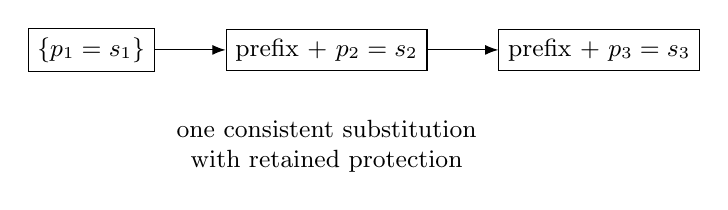
\begin{tikzpicture}[>=Latex,node distance=9mm, every node/.style={font=\small}]
\node[draw] (one) {$\{p_1=s_1\}$};
\node[draw,right=of one] (two) {prefix + $p_2=s_2$};
\node[draw,right=of two] (three) {prefix + $p_3=s_3$};
\draw[->] (one)--(two); \draw[->] (two)--(three);
\node[below=5mm of two,align=center] {one consistent substitution\\with retained protection};
\end{tikzpicture}
\end{center}

This removes repeated term traversal. It does not eliminate the number of
candidate combinations or the size of the requested answer bag. Current
prefix snapshots also copy binding and occurrence metadata, so arbitrarily
wide joins are not promised constant work per added premise. In HE a joint
query computes its complete finite set of answers before returning them; PeTTa
can return answers one at a time.

The checked model concerns first-order matching with a declared equality for
leaves. Binder-aware higher-order matching needs a separate treatment of
scope, equality, search and resources. No higher-order completeness claim
follows from these tests. Machine-checked Lean proofs establish the laws of
the mathematical model; they are not needed at run time, and they do not
verify the compiled C program as a whole.

An interrupted search is not a completed empty search. Check the process and
completion outcome when running bounded experiments; do not feed an
unfinished frontier into a proof or evidence consumer as if it were complete.

Appendix~\ref{app:repro} lists the commands that check these claims and
records one measurement of the prefix reuse.

\section{Exercises with counterexamples}
\begin{enumerate}
\item Add \name{(fact da (edge dana alice))}. Compare bounded answers at
depth four and eight. Which new proofs repeat a vertex? Does rejecting such
proofs preserve all paths, all reachable pairs, or neither?
\item Duplicate \name{(fact ab (edge alice bob))}. Predict the change in
proof multiplicity. Then compare it with the forward client's set-valued
closure. Explain why the different counts are intentional.
\item Add \name{(parent carol $unknown)} to the joint example. Can a later
premise turn that protected variable into a named parent? Construct a
positive shared-variable match and a negative inconsistent one.
\item Replace the raw ancestor test's bound \name{$ancestor} with the
unevaluated expression \name{(car-atom $ancestors)}. Explain why that tests
different syntax and fails to recognize the intended variant.
\item In the evidence example, make both derivations use one observation.
Show that two proof trees do not imply two independent observations.
\item Compare a proof-height budget with Nil's total proof-size budget on a
branching rule. Give a proof admitted by one numeric bound and excluded by
the other when both bounds have the same numeral.
\item Build a small agenda for forward closure. State its duplicate policy
and show that changing the queue order preserves its intended finite
closure. Keep answer order separate from set equality.
\end{enumerate}

\appendix
\section{Reference card}\label{app:card}

All operations below require an \name{extended} profile and, except for
\name{=%}, one \name{!(import! &self pat)}.

\begingroup\small
\begin{longtable}{p{.50\linewidth}p{.44\linewidth}}
\toprule Form & What may bind \\\midrule
\name{(= head body)} & ordinary rule: the head and the caller may both bind\\
\name{(=% head body)} & directional rule: only the head binds; the caller is protected\\
\name{(match space pattern template)} & ordinary retrieval: both sides may bind\\
\name{(pat:match% space pattern template)} & only the pattern binds; stored rows are protected\\
\name{(pat:%match space term $row template)} & only stored rows bind; \name{$row} names each stored row that covers \name{term}\\
\name{(pat:let% pattern producer body)} & evaluate \name{producer}; bind only \name{pattern}\\
\name{(pat:case% producer branches)} & evaluate \name{producer}; each branch pattern binds, the value is protected\\
\name{(pat:unify% pattern subject yes no)} & raw syntax; only \name{pattern} binds\\
\name{(pat:is-instance term pattern)} & test only; ISO \name{subsumes_term(pattern, term)}\\
\name{(pat:is-variant a b)} & test only; one renaming of variables, SWI \name{=@=}\\
\name{(pat:solve policy pairs)} & one witness for several pairs at once; \name{policy} is \name{match%}, \name{%match}, \name{unify} or \name{variant}\\
\name{(pat:apply witness syntax)} & instantiate syntax with a witness\\
\name{(pat:view witness)} & inspect assignments and residual equality constraints\\
\name{(pat:query space policy pattern)} & rows with their occurrence identities and a witness\\
\bottomrule
\end{longtable}
\endgroup

With the rows \name{(edge $stored b)}, \name{(edge a b)} and \name{(edge a b)}:
\name{match} of \name{(edge a $y)} gives three answers, \name{pat:match%} gives
two, and \name{pat:%match} of \name{(edge a b)} returns all three stored rows.

Separate \name{pat:let%} forms are separate attempts: an inner attempt does not
inherit the outer one's protected variables. Use a conjunction pattern or
\name{pat:solve} when several comparisons must share one protected set.

\section{Reproducing the checks and measurements}\label{app:repro}

The maintained checks are:
\begin{code}
make BUILD=python test-pattern test-chaining-tutorial
make BUILD=python test-petta-upstream-profiles PETTA_ORACLE_ROOT=../PeTTa
make BUILD=python test
\end{code}
The pattern gate includes finite-model correspondence, repeated-variable and
alias tests, allocation failures, deliberate defects, and interruption
controls. The tutorial gate independently checks every row of a larger
12-premise proof join, including its duplicate-occurrence combinations.

To collect a scaling record with instruction counts:
\begin{code}
make BUILD=python ENABLE_RUNTIME_STATS=1
python3 scripts/bench_pattern.py --cetta ./cetta \
  --stats-cetta runtime/cetta-python-runtime-stats \
  --reference-cetta path/to/pinned-cetta --samples 5 --instructions \
  --output results/pattern-comparison
\end{code}
Keep a reference executable in its matching repository context so native
libraries resolve correctly. The driver checks answers before accepting a
cost record, identifies its sources and binaries, and alternates execution
order. Compare both same-profile versions and plain versus extended: they
answer different performance questions. A measured finite ladder is evidence
about those clients, not a universal worst-case percentage guarantee.

\subsection{A measured example}
On the qualified GCC 15.2 Python build, five interleaved samples of the
fixed-size prefix workload gave the following median user-instruction counts
(millions). The reference is the directional implementation before prefix reuse;
both executables return the same checked answers.
\begin{center}
\begin{tabular}{rrrrr}
\toprule
Premises & HE reference & HE current & PeTTa reference & PeTTa current\\\midrule
2 & 26.508 & 26.181 & 12.492 & 12.352\\
8 & 34.113 & 32.024 & 12.733 & 12.448\\
32 & 37.970 & 33.045 & 16.902 & 13.611\\
64 & 48.642 & 34.428 & 28.163 & 15.228\\\bottomrule
\end{tabular}
\end{center}
At 64 premises this is about 29\% fewer instructions for HE and 46\% for
PeTTa. The mechanism counters grow by five subject views and six pair visits
per additional premise between the wider rows, after fixed setup work.
The benchmark driver rejects renewed quadratic prefix traversal.

A separate eleven-client chainer ladder uses five balanced samples to compare
each profile against the original pre-directional baseline, and extended
directly against plain. The largest plain-PeTTa median instruction increase
is 0.14\%; extended uses between 0.75\% and 16.93\% fewer instructions than
its baseline. Extended's largest remaining instruction difference from plain
is 0.94\% across this ladder, with identical checked outputs.

For example, backward Loowoz at size 19 uses 32.90 billion instructions in
extended, down from 39.61 billion; the current plain profile uses 32.74 billion.
Compiled calls reuse the ordinary fast path while their definitions remain
unchanged, retaining the existing fallback when declarations change. Compiler,
input shape and machine changes require fresh measurements.

\section*{Sources and companion programs}
\addcontentsline{toc}{section}{Sources and companion programs}
\begingroup\small
The small Horn and closure clients in this guide are explanatory programs.
The larger Nil clients are maintained with pinned provenance in
\nolinkurl{benchmarks/chaining/nil_current/source_provenance.tsv} and their source
headers. The proof-size engine records revision
\nolinkurl{2151416f4d44b3b2dbbcd57a0dd7ffd5a75c992c}; the MM2 semantic-closure examples
record \nolinkurl{9a3287210880ca162beed379942a036a6f3cf8a6}.

\begin{itemize}
\setlength{\itemsep}{0pt}
\setlength{\parskip}{0pt}
\item Nil Geisweiller's chaining experiments:
\url{https://github.com/ngeiswei/chaining}.
\item PeTTa's proof-producing \name{nilbc} example:
\url{https://github.com/trueagi-io/PeTTa/blob/main/examples/nilbc.metta}.
\item The one-sided matching request and the percent convention:
\url{https://github.com/trueagi-io/hyperon-experimental/issues/674}.
\item Executable directional clients and their expected observations:
\name{examples/pattern/}.
\item Reproduction drivers: \nolinkurl{scripts/bench_chaining.py},
\nolinkurl{scripts/bench_pattern.py}, and
\nolinkurl{tests/support/check_chaining_tutorial.py}.
\end{itemize}
\endgroup
\end{document}
